\documentclass[10pt]{article}
\usepackage{amsmath}
\usepackage{tikz}
\usepackage{amsfonts}
\usepackage{enumitem}
\usepackage[math-style=ISO,bold-style=ISO,mathrm=sym]{unicode-math}
\usepackage{pdfpages}
\usepackage{tikz}
\usepackage{xcolor}
\usepackage{xfp}
\usepackage[top=5mm, bottom=2mm, inner=5mm, outer=5mm,
headheight=0mm, headsep=0mm, footskip=0mm,
papersize={210mm, 148mm},
includeheadfoot
]{geometry}
\newcommand{\heading}[1]{
\begin{center}
\setmainfont{Raleway SemiBold}[Scale=1.3]#1
\end{center}\vspace{-7mm}}
\newcommand{\subheading}[1]{
\vspace{-2mm}
\begin{flushleft}
\setmainfont{Raleway SemiBold}[Scale=1]#1
\end{flushleft}\vspace{-5mm}}

\defaultfontfeatures{Ligatures=TeX}
\setmainfont[BoldItalicFont=Linux Biolinum Slanted Bold]{Libertinus Sans}
\setmathfont[NFSSFamily=mathfont,RawFeature={+ss08}]{Libertinus Math}
\DeclareMathAlphabet{\mathcal}{OMS}{cmsy}{m}{n}

% Replace 0-9 with sans serif versions
%\DeclareSymbolFont{MathFont}{TU}{mathfont}{m}{n}
\Umathcode "31 = "0"0"1D7E3
\Umathcode "32 = "0"0"1D7E4
\Umathcode "33 = "0"0"1D7E5
\Umathcode "34 = "0"0"1D7E6
\Umathcode "35 = "0"0"1D7E7
\Umathcode "36 = "0"0"1D7E8
\Umathcode "37 = "0"0"1D7E9
\Umathcode "38 = "0"0"1D7EA
\Umathcode "39 = "0"0"1D7EB
\Umathcode "30 = "0"0"1D7E2


\pagestyle{empty}

\newenvironment{enumerlist}[1][5mm]{\begin{enumerate}[leftmargin=#1]
  \setlength{\itemsep}{1pt}
  \setlength{\parskip}{0pt}
}{\end{enumerate}}
\begin{document}
\noindent\begin{minipage}[t][138mm][t]{95mm}
\heading{Definitions}
\vspace{3mm}
{\footnotesize
\begin{enumerlist}[0mm]
\item[] The \textbf{coefficients} of a polynomial in $x$ are the constants written before each power of $x$. For example,
        the coefficients of \(4x^2+12x+9\) are 4, 12 and 9.
\item[] The \textbf{geometric mean} of a set of \(n\) numbers is the \(n\)th root of the product of the numbers.
\item[] The \textbf{factors} of a number are the numbers that it can be divided by without leaving a remainder.
        1 and the number itself are included as factors in each puzzle where factors are used.
\item[] The \textbf{consecutive integers} starting at 500 are the numbers 500, 501, 502, \dots{}
\end{enumerlist}
}

\vspace{4mm}

\heading{Hints}
\vspace{3mm}
{\footnotesize
\begin{enumerlist}[10mm]
\item[1.] There are 12 different ways that you could make the two 2-digit numbers.
\item[2.] What should the leftmost digit of each number be? Once you've picked a 2-digit number, how should you arrange the digits in the 8-digit number?
\item[3.] \((30x+5)^2 = 900x^2+300x+25\)
\item[4.] How could you do the previous question without expanding the brackets?
\item[5.] The factors of 41306329 are 1, 6427, and 41306329.
\item[6.] What are the geometric means of the factors of the numbers from 1 to 20?
\item[7.] What are the factors of 7? What are the factors of $7^2$? $7^3$?
\item[8.] Which numbers between 1 and 20 have an odd number of factors?
\item[9.] What would the result be if Eve had used 3 consecutive integers? 4? 5?
\item[10.] If you change the 500 in question 9 for a different number, how do you need to change the 365 to keep the answer the same?
\end{enumerlist}
}

%\heading{Solutions}
%\vspace{3mm}
%{\footnotesize
%
%}
\vfill
\begin{center}\footnotesize
\includegraphics[width=.14\textwidth]{scorpion.png}
\\
\includegraphics[width=.75\textwidth]{logo.jpg}
\\
\begin{minipage}{3.5cm}
chalkdustmagazine.com
\\
@chalkdustmag
\\
\#ChalkdustChristmasCard2025
\end{minipage}
\end{center}
\end{minipage}\hspace{10mm}\begin{minipage}[t][138mm][t]{95mm}
\vspace*{-1mm}

\begin{center}
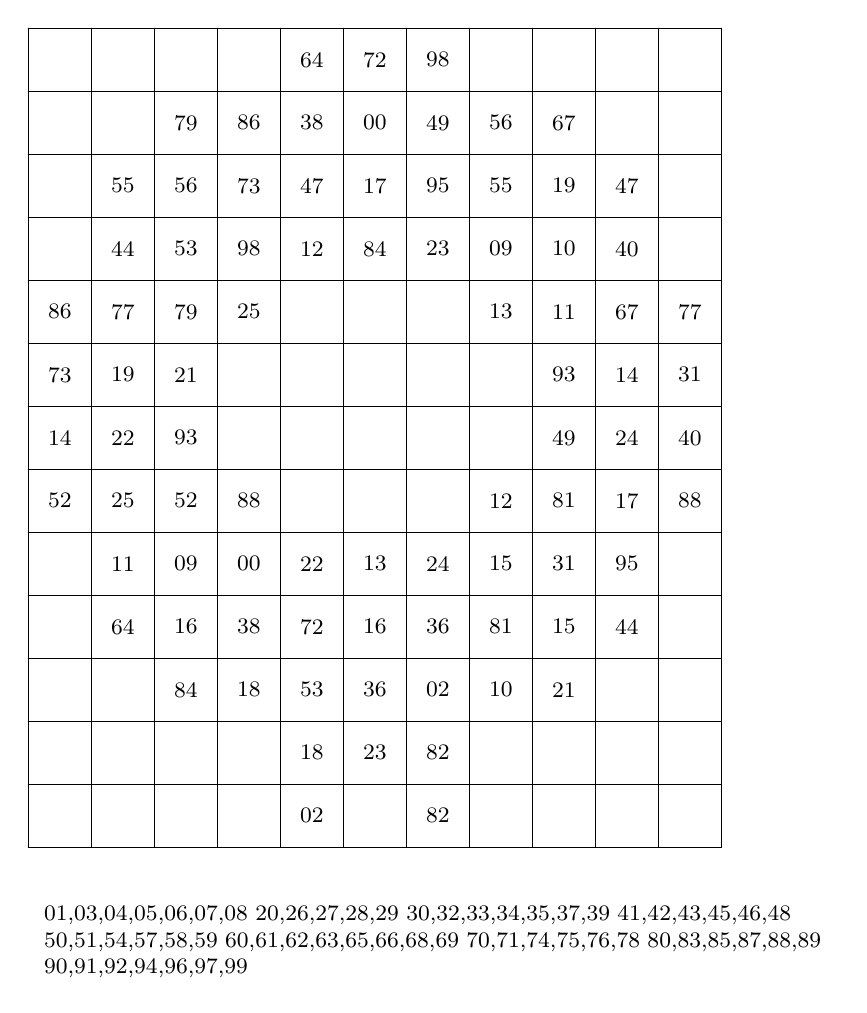
\begin{tikzpicture}[y=8mm,x=8mm,line width=0.5pt,line cap=round,line join=round]
\footnotesize
\begin{scope}[shift={(0.5,0.5)}]
\node[text width=10cm] at (6,-2) {
01,03,04,05,06,07,08
20,26,27,28,29
30,32,33,34,35,37,39
41,42,43,45,46,48
50,51,54,57,58,59
60,61,62,63,65,66,68,69
70,71,74,75,76,78
80,83,85,87,88,89
90,91,92,94,96,97,99
};
\node at (5,2) {36};\node at (6,3) {36};

\node at (8,6) {49};\node at (6,11) {49};
\node at (2,6) {93};\node at (8,7) {93};
\node at (3,3) {38};\node at (4,11) {38};
\node at (8,5) {81};\node at (7,3) {81};
\node at (5,10) {17};\node at (9,5) {17};
\node at (5,12) {72};\node at (4,3) {72};
\node at (3,5) {88};\node at (10,5) {88};
\node at (2,2) {84};\node at (5,9) {84};

\node at (5,4) {13};\node at (7,8) {13};

\node at (3,8) {25};\node at (1,5) {25};
\node at (0,5) {52};\node at (2,5) {52};
\node at (2,7) {21};\node at (8,2) {21};

\node at (7,5) {12};\node at (4,9) {12};
\node at (5,1) {23};\node at (6,9) {23};

\node at (6,12) {98};\node at (3,9) {98};
\node at (0,8) {86};\node at (3,11) {86};
\node at (4,12) {64};\node at (1,3) {64};
\node at (10,6) {40};\node at (9,9) {40};
\node at (7,9) {09};\node at (2,4) {09};

\node at (1,4) {11};\node at (8,8) {11};

\node at (9,7) {14};\node at (0,6) {14};
\node at (9,3) {44};\node at (1,9) {44};
\node at (4,10) {47};\node at (9,10) {47};
\node at (3,10) {73};\node at (0,7) {73};
\node at (8,4) {31};\node at (10,7) {31};
\node at (1,7) {19};\node at (8,10) {19};
\node at (9,4) {95};\node at (6,10) {95};
\node at (7,10) {55};\node at (1,10) {55};
\node at (2,10) {56};\node at (7,11) {56};
\node at (9,8) {67};\node at (8,11) {67};
\node at (1,8) {77};\node at (10,8) {77};
\node at (2,8) {79};\node at (2,11) {79};

%%%%%%%%%%%%%%%% RED %%%%%%%%%%%%%%%%%%%

\node at (2,3) {16};\node at (5,3) {16};

\node at (7,2) {10};\node at (8,9) {10};
\node at (3,4) {00};\node at (5,11) {00};
\node at (6,2) {02};\node at (4,0) {02};

\node at (8,3) {15};\node at (7,4) {15};
\node at (2,9) {53};\node at (4,2) {53};

\node at (3,2) {18};\node at (4,1) {18};
\node at (6,0) {82};\node at (6,1) {82};
\node at (4,4) {22};\node at (1,6) {22};
\node at (6,4) {24};\node at (9,6) {24};

\end{scope}



%\foreach \x/\y in {
%    5/1,
%    2/2,5/2,8/2,
%    1/3,3/3,4/3,6/3,7/3,9/3,
%    1/4,2/4,5/4,8/4,9/4,
%    0/5,1/5,2/5,3/5,7/5,8/5,9/5,10/5,
%    0/6,2/6,8/6,10/6,
%    0/7,1/7,2/7,8/7,9/7,10/7,
%    0/8,1/8,2/8,3/8,7/8,8/8,9/8,10/8,
%    1/9,3/9,4/9,5/9,6/9,7/9,9/9,
%    1/10,2/10,3/10,4/10,5/10,6/10,7/10,8/10,9/10,
%    2/11,3/11,4/11,6/11,7/11,8/11,
%    4/12,5/12,6/12
%}
%    \fill[green] (\x,\y) rectangle +(1,1);
%\foreach \x/\y in {
%    4/0,6/0,
%    4/1,6/1,
%    3/2,4/2,6/2,7/2,
%    2/3,5/3,8/3,
%    3/4,4/4,6/4,7/4,
%    1/6,9/6,
%    2/9,8/9,
%    5/11
%}
%    \fill[red] (\x,\y) rectangle +(1,1);

\foreach \x in {0,...,11}
    \draw (\x,0) -- +(0,13);
\foreach \y in {0,...,13}
    \draw (0,\y) -- +(11,0);

\end{tikzpicture}

\end{center}

\vfill
\begin{center}
{\setmainfont[Scale=3]{Pacifico}Merry Christmas}\\
{(instructions inside)}
\end{center}
\vfill\null
\end{minipage}

\newpage

\noindent\begin{minipage}[t][138mm][t]{95mm}
\heading{Instructions}
\vspace{3mm}
{\footnotesize
\begin{enumerlist}
\item Solve the puzzles below.
\item Each answer will have an even number of digits. Form a sequence of numbers by splitting the answer into pairs of digits, then join the dots on the front
      of the card following the sequence. For example, if the answer to a puzzle were 77031827, you would draw straight lines
      from dot 77 to dot 3, from dot 3 to dot 18, and from dot 18 to dot 27.
\item Colour any region containing an even number of unused dots green. Colour any region containing an odd number of unused dots red or blue.
\end{enumerlist}}

\vspace{5mm}

\heading{Puzzles}
{\footnotesize
\begin{center}\footnotesize(see back of card for definitions and hints)\end{center}\vspace{-3mm}
%1. 13 12
%2. 84 04 14 81 60
%3. 12 25
%4. 17 71 47
%5. 64 27
%6. 84 64
%7. 28 01
%8. 17 02 60
%9. 13 32 25
%10. 47 27
\begin{enumerlist}
\item[1.] What is the largest number you can make by using the digits 1 to 4 to make
          two 2-digit numbers, then mutiplying the two numbers together?
\item[2.] What is the largest number you can make by using the digits 0 to 9 to make
          a 2-digit number and a 8-digit number, then mutiplying the two numbers together?
\item[3.] The expansion of \((2x+3)^2\) is \(4x^2+12x+9\). The sum of the coefficients of
          \(4x^2+12x+9\) is 25. What is the sum of the coefficients of the expansion of \((30x+5)^2\)?
\item[4.] What is the sum of the coefficients of the expansion of \((2x+1)^{11}\)?
\item[5.] What is the geometric mean of all the factors of 41306329?
\item[6.] What is the largest number for which the geometric mean of all its factors is 92?
\item[7.] What is the sum of all the factors of \(7^4\)?
\item[8.] How many numbers between 1 and 28988500000 have an odd number of factors?
\item[9.] Eve found the total of the 365 consecutive integers starting at 500 and the total of the next 365 consecutive integers,
          then subtracted the smaller total from the larger total. What was her result?
\item[10.] Eve found the total of the \(n\) consecutive integers starting at a number and the total of the next \(n\) consecutive
           integers, then subtracted the smaller total from the larger total. Her result was 22344529.
           What is the largest possible value of \(n\) that she could have used?
\end{enumerlist}
}
\end{minipage}\hspace{10mm}\begin{minipage}[t][138mm][t]{95mm}
\vfill
\begin{center}
{\setmainfont[Scale=3]{Pacifico}Merry Christmas}\\
\end{center}
\vfill
\begin{center}
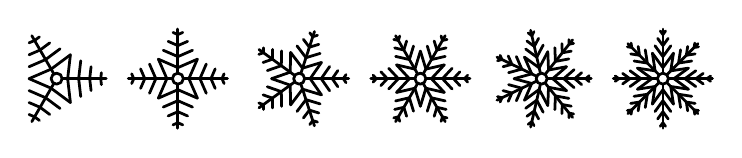
\begin{tikzpicture}[x=7mm,y=7mm,line cap=round,line join=round,line width=1pt]
\foreach \n in {3,...,8} {
\begin{scope}[shift={(2.2*\n,0)}]
\draw (0,0) circle (0.1);
\foreach \i in {1,...,\n} {
    \begin{scope}[rotate=360*\i/\n]
        \draw (0.1,0) -- (0.9,0);

        \foreach \a in {1, 2, 3, 4}
        \draw
            (0.2*\a,0) -- +({(5/4-\a/4)*(0.5*cos(180/\n)-0.2)},{(5/4-\a/4)*0.5*sin(180/\n)})
            (0.2*\a,0) -- +({(5/4-\a/4)*(0.5*cos(180/\n)-0.2)},{-(5/4-\a/4)*0.5*sin(180/\n)});
        %\foreach \a in {1, 2, 3, 4}
        %\draw
        %    (0.03+0.15*\a,0) -- +({0.05*(5-\a)},{0.05*(5-\a)})
        %    (0.03+0.15*\a,0) -- +({0.05*(5-\a)},{-0.05*(5-\a)});
    \end{scope}

}
\end{scope}
}
\end{tikzpicture}
\end{center}
\vspace{1mm}
\end{minipage}


\end{document}

